%This file contains the tex code of my project report for my Data Structure course.
%Author: 章凌豪 / Zhang Linghao <zlhdnc1994@gmail.com>

\section{问题分析}

\subsection{问题描述}

\begin{itemize}
\item 给定一个有$N(N\leq10^{7})$个表项的IPv4(或IPv6)地址路由表
\item 给出$M(M\leq10^{6})$个操作,每个操作是下列三种之一:
\begin{itemize}
\item 查找一个IP地址所对应的下一跳端口
\item 插入(若已存在则修改)一条路由表项
\item 删除一条路由表项
\end{itemize}
\end{itemize}

\subsection{要点分析}

\begin{itemize}
\item 路由转发是一个最长匹配前缀查找的过程。
\item 需要一个动态的数据结构来支持更新操作(包括增加、修改和删除),并且更新的复杂度不能太高。
\item 由于$N$较大,算法的时间复杂度最好与$N$无关。
\item 考虑到将算法拓展到IPv6地址的情形,需要考虑算法的时空复杂度是否依赖于IP地址位数$W$。
\end{itemize}

\subsection{Trie简介}

Trie,又称前缀树或字典树,是一种用于动态维护字符串的数据结构。字符串的最长匹配前缀查找就是Trie的经典应用之一。\\
\indent
在本问题中,IP地址相当于01字符串,所以解决本问题的一种最朴素的方法就是使用Binary Trie。\\
\indent
图1是将$P1$到$P9$的前缀插入Binary Trie后形成的结构。整个Binary Trie是一棵二叉树,图中的每个黑色结点都对应着一个前缀。查询操作即是从根结点按待查IP地址的对应二进制位选择左分支或右分支往下走,记录下最后一个遇到的黑色结点,其对应的前缀便是该IP地址的最长匹配前缀。更新操作则是先找到对应的结点,再将其标为黑色或标回白色。其中插入时有可能要创建新结点。\\
\indent
显然查询和更新操作都十分容易实现,且都能在$O(depth)$内完成。但简单的代价就是在最坏情况下每次操作都要走到树的最底层,可能导致性能表现不佳。而在真实世界的路由表中,/24的前缀最为常见,这意味着树的深度一般都会超过$24$。除此之外,Binary Trie中存在大量无效结点,空间使用效率极低。它在IPv4下的表现或许还不错,到了IPv6下由于地址长度增为原来的$4$倍,空间使用呈指数式上升,实用性不强。\\
\indent
朴素的Binary Trie的这些缺点催生了它的许多变种,比如我们熟知的通过将连续的白色结点压缩从而节省空间和缩短搜索路径的Path Compression Trie等。在这些变种中有一种叫做Multi-bit Trie,本报告将在第2节详述的Dynamic Tree Bitmap就是基于它发展而来的。\\
\indent
Multi-bit Trie的主要思想是通过将连续$stride$(之后简记为$S$)个结点压缩成一个结点,从而将Trie的高度从$W$压缩到$\lceil\frac{W}{S}\rceil$,达到压缩查询路径的目的。图2是图1的例子在Multi-bit Trie上形成的结构,可以看到树的高度从$5$被压缩到$2$。由于涉及到前缀扩展(prefix expansion),Multi-bit Trie的更新花费是$O(\lceil\frac{W}{S}\rceil + 2^{S})$的,空间花费为$O(\frac{2^{S}NW}{S})$。Multi-bit Trie虽然在查询上很理想,但更新花费过大,所以不适合本问题中需要面对的高度动态情形。\\

\begin{figure}[h!]
\centering
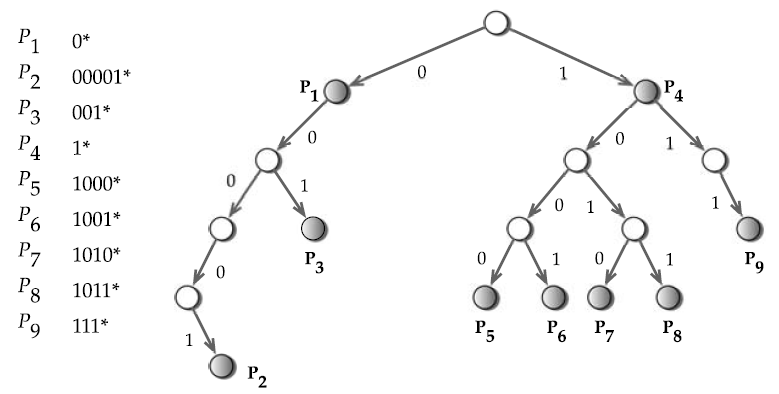
\includegraphics[scale=0.4]{trie.png}
\caption{图1}
\end{figure}

\begin{figure}[h!]
\centering
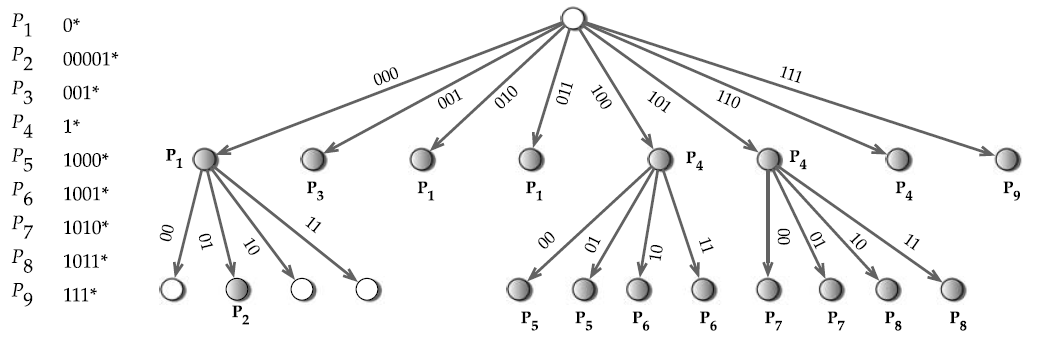
\includegraphics[scale=0.4]{mbt.png}
\caption{图2}
\end{figure}

\clearpage